\documentclass[a4paper]{article}

%% Language and font encodings
\usepackage[english]{babel}
\usepackage[utf8x]{inputenc}
\usepackage[T1]{fontenc}

%% Sets page size and margins
\usepackage[a4paper,top=3cm,bottom=2cm,left=3cm,right=3cm,marginparwidth=1.75cm]{geometry}

%% Useful packages
\usepackage{amsmath}
\usepackage{graphicx}
\usepackage[colorinlistoftodos]{todonotes}
\usepackage[colorlinks=true, allcolors=blue]{hyperref}

\title{IF686 - Paradigmas de Linguagens Computacionais}
\author{Lucas e Silva de Souza}

\begin{document}
\maketitle

\begin{figure}[ht]
\centering
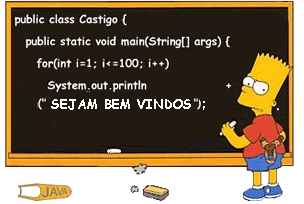
\includegraphics[width=0.5\textwidth]{lss8.jpg}
\caption{\label{fig:download}Bart aprendendo um jeito mais fácil de cumprir a sua punição.}
\end{figure}

\section{Introdução}

\paragraph{} A disciplina IF686 se encaixa na área de programação e computação básica, ela ensina, como o próprio nome já diz, paradigmas de linguagens de programação, mais especificamente, o paradigma funcional(com ênfase em Haskell) e o concorrente(com ênfase em Java). 
\paragraph{} A ideia é fazer com que os alunos aprendam a utilizar de maneira eficiente outros paradigmas, fora o imperativo, além de adquirir um conhecimento mais refinado nas estruturas de construção usadas nessas linguagens. Os alunos também devem obter uma visão mais impessoal e crítica sobre as diversas linguagens de programação, reconhecendo seus pontos positivos e negativos, para que possam escolher a "ferramenta" mais apropriada para resolver o problema em mãos.  

\subsection{Paradigma Funcional}

\paragraph{} A programação funcional é baseada no uso de funções, dessa forma evita mudança em dados ou estados do programa, ao contrario da programação imperativa. Atualmente tem sido mais usada academicamente que comercialmente. 

\subsection{Paradigma Concorrente}

\paragraph{} A programação concorrente faz uso de uma execução simultânea de tarefas computacionais diferentes, sendo implementadas como um conjunto de vários programas, ou por parte de threads geradas por um único programa.

\newpage
\section{Relevância}

\paragraph{} A disciplina aumenta o conhecimento do aluno em um aspecto fundamental do curso, que é a habilidade de programação, além de melhorar o senso crítico e a visão que o estudante tem sobre diversas linguagens e paradigmas da programação. Através do conhecimento adquirido, o aluno será um profissional com melhor capacidade para escolher a melhor "ferramenta" para resolver de maneira mais eficiente possível qualquer tarefa que necessitar.

\paragraph{} Ela também é a disciplina base caso algum aluno deseje se aprofundar mais nos estudos de programação, sendo pré-requisito de diversas cadeiras de desenvolvimento de software e tipos específicos de programação. Resumindo :

\begin{itemize}
\item Melhora habilidade de programação
\item Ajuda o aluno a pensar de maneira diferente
\item Ensina paradigmas alternativos
\item Mostra novas linguagens computacionais
\end{itemize}

\section{Relação com outras disciplinas}

\begin{table}[ht]
\begin{tabular}{|l|l|}
\hline
IF710 - Programação com Componentes           & \begin{tabular}[c]{@{}l@{}}Continua os estudos do paradigma concorrente, mas mais \\ especificamente a programação com uso de componentes.\end{tabular}                                \\ \hline
IF708 - Programação Funcional                 & \begin{tabular}[c]{@{}l@{}}Essa disciplina vai estudar com mais profundidade o \\ paradigma funcional, visto de forma mais básica \\ na disciplina IF686.\end{tabular}                 \\ \hline
IF734 - Projeto de Compiladores               & \begin{tabular}[c]{@{}l@{}}Apresenta uma introdução a Domain-Specific Language \\ (DSL),  que são os paradigmas e funções específicos \\ de uma linguagem de programação.\end{tabular} \\ \hline
IF711 - Programação Concorrente e Distribuída & \begin{tabular}[c]{@{}l@{}}Utiliza notação de alto nível para mostrar aspectos \\ de concorrência e distribuição no desenvolvimento \\ de softwares.\end{tabular}                      \\ \hline
\end{tabular}
\end{table}

\section{Referências}

\paragraph{} Os livros-texto da disciplina são o Learn You a Haskell for Great Good!\cite{lipovaca2011learn} e Java Concurrency in Practice\cite{bloch2017effective}. Além deles, outros livros indicados pelo professor são o Haskell: The Craft of Functional Programming\cite{thompson2011haskell}, para programação funcional, o Parallel and Concurrent Programming in Haskell\cite{marlow2012parallel}, para programação concorrente, e o Programming Language Pragmatics\cite{scott2000programming}. 

\bibliographystyle{alpha}
\bibliography{lss8}

\end{document}